\chapter{System Design}

\section{System Overview}

The vending machine system consists of three main parts, namely the QR Code component, the NFC
component and the actual vending machine. 

Figure \ref{fig:system-overview-pi} and \ref{fig:system-overview-machine} gives a
diagrammatical layout of the complete system.
It shows the interactions between the different sub-components of the complete system.

\begin{figure}[h]
\centering
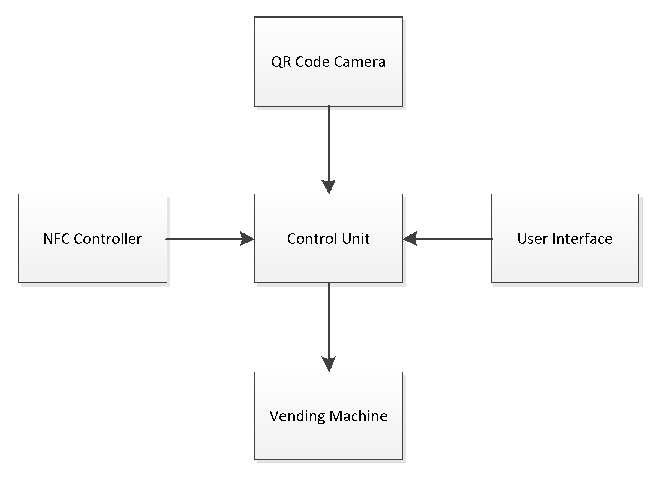
\includegraphics[scale=0.7]{pi_system_overview.eps}
\caption{System overview from the control unit's perspective}
\label{fig:system-overview-pi}
\end{figure}

\begin{figure}[h]
\centering
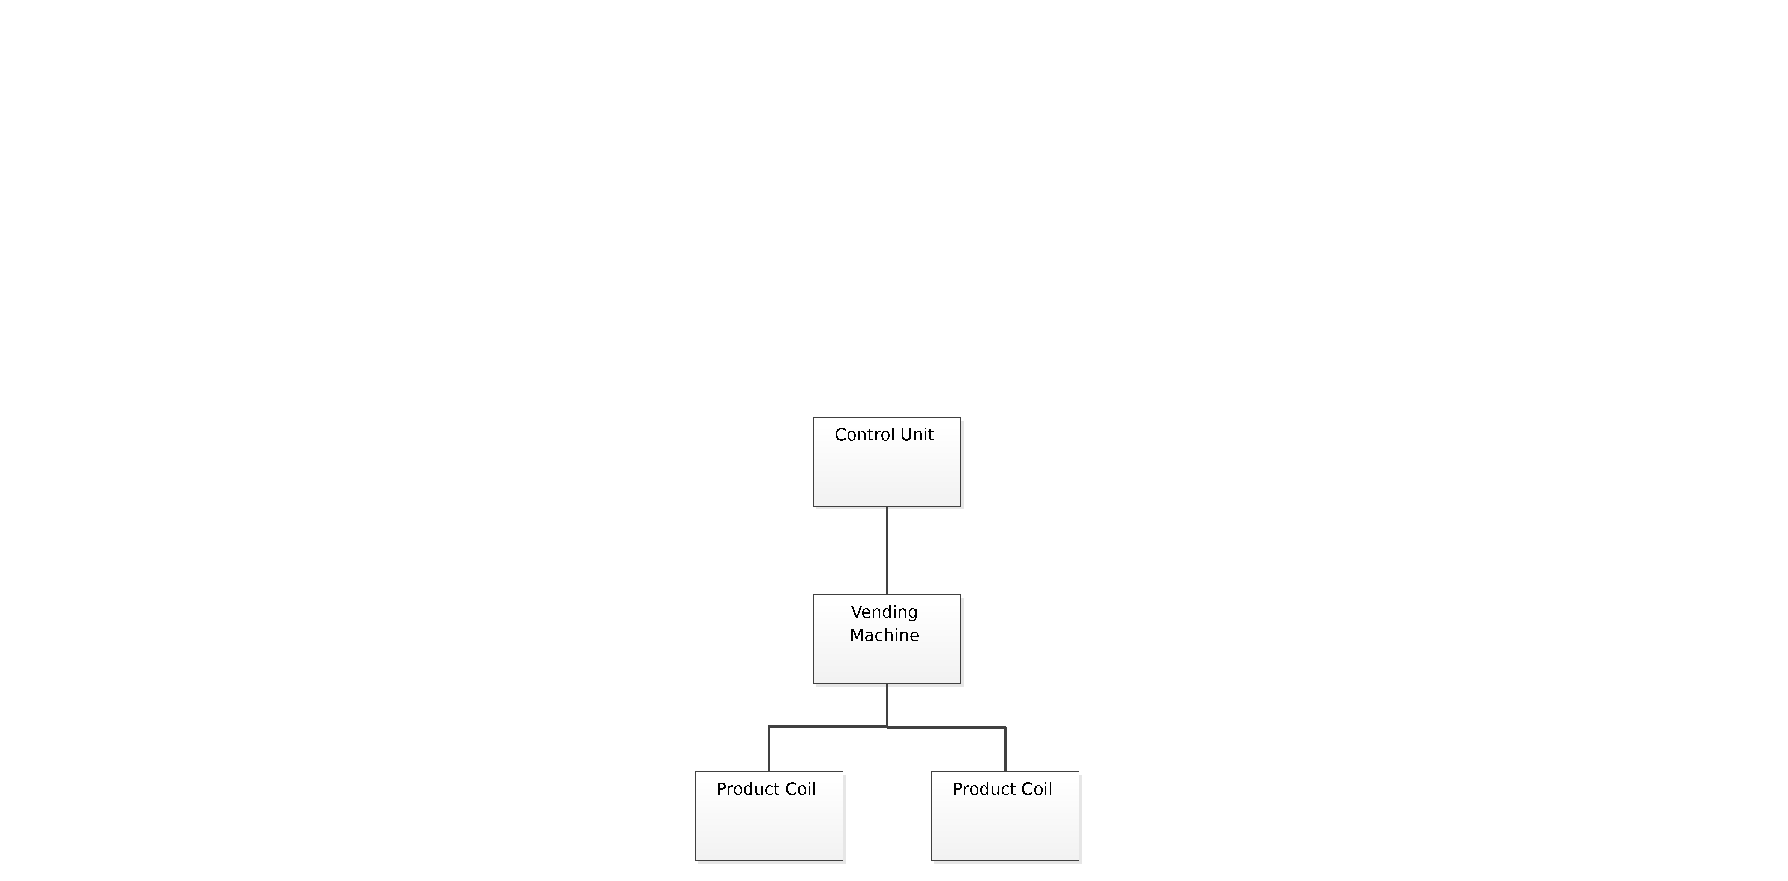
\includegraphics[trim=5cm 0 0 6cm, clip=true,
scale=0.7]{vending_machine_system_overview.eps}
\caption{System overview from the vending unit's perspective}
\label{fig:system-overview-machine}
\end{figure}

It can be seen that the complete system is divided up into five main parts, namely 

\begin{enumerate}
  \item Control unit.
  \item NFC controller.
  \item QR Code camera.
  \item Vending machine unit.
  \item Vending machine coils.
\end{enumerate}

The components used in these subsystems are discussed in the subsequent sections of this
chapter.

\section{Central Control Unit}

To be able to handle the image processing that QR Code decoding and NFC handling requires, a
relatively powerful central controller is required. Although there are many controllers capable
of this, only two main alternatives were considered in this project. They are the Raspberry Pi microcomputer and
the Arduino Uno microcontroller.

\subsection{Arduino Uno}

The Arduino Uno is popular open-source microcontroller (see Figure \ref{fig:arduino}). 

\begin{figure}[h]
\centering
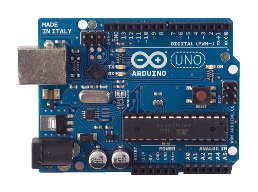
\includegraphics[scale=1.5]{arduino.eps}
\caption[Picture of an Arduino Uno microcontroller]{Picture of an Arduino Uno microcontroller
[\cite{manual:arduino-specs}]}
\label{fig:arduino}
\end{figure}

It is
based on the 8-bit Atmel ATmega328 ARM microprocessor. Its official specifications are [\cite{website:arduino-specs}]:

\begin{tabbing}

Operating Voltage: \= 5 V \\ 
Processor: \> Atmel ATmega328 (clocked at 16 MHz) \\
GPIO Pins: \> 14 (6 of which are PWM enabled) \\
Memory: \> 32 kB Flash, 2kB SRAM, 1kB EEPROM \\
Communication: \> $i^2c$, UART, SPI. \\
Price: \> R310.00 \\

\end{tabbing}

Because of its open-source design, there are a multitude of peripheral devices and expansion
boards (known as `shields'), along with all their libraries and drivers, available locally. The
Arduino's programming language of choice is a modified, but remarkably simple, version of C
and comes with its own Integrated Development Environment (IDE). This, along with its relatively low cost and adequate
specifications, makes the Arduino Uno an attractive option for this project.

\subsection{Raspberry Pi}

The Raspberry Pi is a Debian Linux-based microcomputer
designed and manufactured by a UK-based charity called the Raspberry Pi Foundation, for the
purpose of educating and familiarising young children with programming. However, its low price
and respectable specifications makes it a strong choice for for a control unit for the vending
machine.

The Pi is made with the focus on Python as its main programming language, which makes running
scripts and controlling the board relatively simple. It also runs on a modified version of
Debian Linux called Raspbian.

Its main specifications are [\cite{website:raspi-specs}]:

\begin{tabbing}

Communication: \= SPI, UART, USB, $i^2c$, Ethernet \\ 
Memory: \> 512 MB RAM \\
Processor: \> ARM 6 clocked at 700 MHz \\
Video: \> HDMI video output \\
GPIO: \> 28 pins \\
Price: \> R400.00 \\

\end{tabbing} 

The Raspberry Pi was chosen to be used as the central controller of this project and
controls the hardware connected to it via a Universal Serial Bus (USB) connection, or one of
its General Purpose Input Output (GPIO) pins.

The Pi was chosen instead of the Arduino Uno for the following reasons:

\begin{itemize}
  
  \item The Pi has more processing power (700MHz vs 16MHz).
  \item The Pi's ability to easily interface with desktop computer peripheral hardware,
  such as a keyboard, mouse and webcam.
  \item The excellent support structure in place and the information on existing and ongoing
  projects that are available on the internet.
  \item The Pi can output its video feed to a computer screen, which makes it possible to
  add a simple user interface (GUI) for uder interaction. 

\end{itemize}

Stated simply, the Raspberry Pi is a compact, traditional desktop computer which makes it very
easy to work with, and its low price makes it an excellent choice for use as the central
controller for the vending machine.

\section{NFC Controller}

The NFC controller that was selected is the PN532 NFC shield from Adafruit Industries
[\cite{website:adafruit-nfc}]. It is based on
the Phillips PN532 chip, which is a widely used NFC chip. The main reason it was selected ahead
of other NFC controllers was that it has a large support base in the open source
community and is fully compatible with the libnfc open-source NFC library
[\cite{website:libnfc-hardware}]. The manufacturer (Adafruit, inc.) also provides comprehensive
documentation and guides on how to set up and configure the controller.
 
The main purpose of this component is to add the option of sending or receiving data through a NFC connection.
This component is also capable of reading RFID cards, such as student or staff cards, as NFC
and RFID transmit similar types of data. This adds the option of paying for the products with 
any NFC-capable smart phone running Google's Android operating system, or with a SU staff or
student card.

\section{QR Code Camera}

To decode QR Codes, the vending machine needs to take pictures of a code so that it can be
decoded using the ZBar library. A PlayStation 2 EyeToy was chosen and added to the system to
facilitate this. It was chosen for the following reasons:

\begin{itemize}
  \item Its drivers are freely available for Linux systems [\cite{website:webcam-drivers}].
  \item Interfaces easily with the USB ports on the Pi.
  \item There was one lying in the supply cupboard.
\end{itemize}

There is currently a camera add-on available for the Raspberry Pi, but this is relatively
expensive and (approximately \$30 [\cite{website:raspi-camera}] versus the Pi's \$35), at the
time of writing, unavailable in South Africa.

\section{Product Dispensing}

\subsection{Coils}

To be able to effectively dispense bought products to the user, a traditional coil mechanism is
used. Such systems are the most familiar and simple methods of dispensing goods. See Figure
\ref{fig:vm-coils} for an example.

\begin{figure}[h]
\centering
\includegraphics[scale=0.2]{vm_coils.eps}
\caption{Example of vending machine coil system [\cite{website:arduino-specs}]}
\label{fig:vm-coils}
\end{figure}

These coils are designed and made in such a manner that one rotation of the coil will drop one
product. The turning motion is made by attaching a DC motor to the base of the coil (see
section \ref{sec:dc-motor} for a more detailed description).

\subsection{DC Motors}
\label{sec:dc-motor}

The motors attached to the base of the coils are two 12V DC mootors from Faulhaber
[\cite{manual:dc-motors}]. Although these motors are rated for 12V, it is possible to run them
from a lower voltage. This will cause the motor to turn slower, and therefore be easier to
control. 

The motors are switched on by a 12V relay switch controlled by the Raspberry Pi. See section
\ref{sec:relay-switch} for more detail about the switch.

\subsection{Relay Switch}
\label{sec:relay-switch}

A relay is a type of electronic switch, which means that it acts like a normal switch, but
requires a voltage across it to open or close it. With this it is possible to control when the
DC motors turn (after a successful transaction) and when they are standing still. 

However, the relays used here are 12V. The Raspberry Pi can deliver a maximum of 5V. Therefore
it was decided that the relay will be permanently connected to a 12V DC supply, but will be
switched by a 2N2222 transistor, which is controlled directly from the Pi's  GPIO pins (see
section \ref{sec:detail-switch} for a detailed discussion).

This allows the Pi to directly control the motors and due to the circuits construction, the Pi
is protected from the relatively high voltages and currents involved in the working of the
motor nd relay.

\section{Vending Machine Unit}

The vending machine unit houses all the components (i.e. the Raspberry Pi, the NFC Shield,
webcam, switches, motors and the product coils). Its made of 1.6mm mild steel plate and was
made by Fabrinox, Paarl. See Appendix \ref{app:vm-tekeninge} for detailed manufacturing
drawings.
